%\documentclass[manuscript]{geophysics}
%\usepackage[nomarkers]{endfloat}

% For a two-column format that looks like the final product, uncomment bellow
% and comment the two lines above
\documentclass[paper,twocolumn,twoside]{geophysics}

\usepackage{graphicx}

\usepackage{amsmath}
\usepackage{array}

\usepackage{booktabs}
\usepackage{color}
\usepackage{epstopdf}

\newcommand{\vect}[1]{\mathbf{#1}}
\newcommand{\mat}[1]{\mathbf{#1}}
\newcommand{\comp}[1]{#1^{\alpha\beta}}
\newcommand{\norm}[1]{\left|\left|#1\right|\right|}

\begin{document}

\title{Gravitational disturbance}

% manuscript number
\ms{GEO-2015-XXXX}

\address{
    \footnotemark[1]
    Observat\'{o}rio Nacional, Rio de Janeiro, Brazil \\
    \footnotemark[2]
    Universidade do Estado do Rio de Janeiro, Rio de Janeiro, Brazil \\
    e-mails: vandscoelho@gmail.com, valcris@on.br

}

\author{Vanderlei C. Oliveira Jr.\footnotemark[1],
Leonardo Uieda\footnotemark[2] and
Val\'{e}ria C. F. Barbosa\footnotemark[1]}

\lefthead{Oliveira Jr., Uieda and Barbosa}
\righthead{Gravitational disturbance}

%%%%%%%%%%%%%%%%%%%%%%%%%%%%%%%%%%%%%%%%%%%%%%%%%%%%%%%%%%%%%%%%%%%%

\begin{abstract}

Gravity anomalies have long been used by geophysicists for the 
purpose of determining density distributions in subsurface.

However, gravity anomalies 

In this paper, we discuss the fundamental concepts 

URGENTE: \citep{marussi1974}, \citep{torge2012}, section 4.2.1

\end{abstract}

%%%%%%%%%%%%%%%%%%%%%%%%%%%%%%%%%%%%%%%%%%%%%%%%%%%%%%%%%%%%%%%%%%%%

\section{Introduction}


The resultant of gravitational force and centrifugal force acting 
on a body at rest on the Earth's surface is called gravity vector
and its intensity is called simply gravity 
\citep{hofmann-wellenhof-moritz2005}.
In the case of gravimetry on moving platforms (e.g., airplanes,
helicopters, marine vessels), there are additional
non-gravitational accelerations due to the vehicle motion, 
such as Coriolis acceleration and high-frequency vibrations 
\citep{glennie-etal2000, nabighian-etal2005-grav, baumann_etal2012}.
Gravity is the most commonly measured quantity in
geophysical surveying.
Geophysicists use gravity for estimating the Earth's 
internal density distribution whereas geodesists use
gravity to estimate the geoid \citep{li2001}
Hence, geophysicists are usually interested 
in the gravitational component of the observed gravity 
which is produced by the Earth's internal 
density distribution.
The first step of the procedure for isolating the
gravitational component of the observed gravity 
consists in removing the non-gravitational effects due 
to the vehicle motion and also the time variations
such as Earth tides, instrumental drift and barometric 
pressure changes, for example.
If these effects are properly removed, the resultant 
gravity data can be considered as the sum of a 
centrifugal component due to the Earth's rotation and
a gravitational component produced by the whole Earth's
internal density distribution.
%For simplicity, we will henceforth call this 
%resultant gravity corrected from non-gravitational 
%effects due to the vehicle motion and also time variations
%as simply gravity.

In applied geophysics, gravity surveys are usually conducted 
over small areas on the Earth's surface for the purpose of 
characterizing geological structures located within the
crust and upper mantle.
Consequently, geophysicists are only interested in the
particular gravitational component of gravity which 
is produced by these target geological structures.
The isolation of this particular gravitational component 
and its subsequent use for estimating density 
distributions related to geological structures in subsurface 
are the main goals in applied geophysics 
\citep{blakely1996}.

In this paper, we discuss the theoretical definition
of the gravitational disturbance based on the 
well-established concepts of normal Earth, normal gravity, 
gravity disturbance and gravity anomalies.
The concept of gravitational disturbance plays an
important role in the discussions about 
the use of gravity disturbance or gravity anomalies
in geophysical applications.
It seems that this theoretical issue has been 
debated within the scientific community from a 
more geodetic than geophysical point of view
\citep{lafehr1991, chapin1996, li2001, fairhead2003,
hackney-featherstone2003, hinze2005}.
Our reasoning suggests that the gravity 
disturbance is conceptually more appropriated than 
gravity anomalies for approximating
the gravitational disturbance and use it for estimating 
density distributions in subsurface.


\section{Normal Earth and normal gravity}


Traditionally, the Earth's gravity field is approximated 
by the gravity field produced by a geocentric and rigid ellipsoid 
of revolution which has the minor axis $b$ 
coincident with the mean rotating axis of the Earth $Z$, the 
same total mass (including the atmosphere) and also the
same angular velocity of the Earth (Figure \ref{fig:fig1}).
Another characteristic of this model is that its
limiting surface coincides with a particular equipotential 
of its own gravity field.
This model is called as normal Earth and its gravity
field is called normal gravity field
\citep{vanicek1987, hofmann-wellenhof-moritz2005, torge2012}.


It is worth noting that, although the normal Earth has the
same total mass (including the atmosphere) of the Earth,
its internal density distribution is unknown.


The only condition imposed on its internal density
distribution is that it produces a normal gravity field
having a particular equipotential which coincides
with its limiting surface.


For convenience, we denote any density distribution 
satisfying this condition as a normal density distribution.




The normal Earth gives rise to the geodetic coordinate system.
In this coordinate system, the position of a point $P$
is defined by the geometric height $h$, geodetic latitude
$\varphi$ and longitude $\lambda$ (Figure \ref{fig:fig1}).
Geodetic coordinates $(h, \varphi, \lambda)$ can be easily 
converted into geocentric Cartesian coordinates $(X, Y, Z)$
(Figure \ref{fig:fig1}).
The plane containing the point $P$, the axis $Z$ and
the origin $O$ of this geocentric Cartesian coordinate system
is called meridian plane (gray plane in Figure \ref{fig:fig1}).


Similarly to the gravity vector and gravity, 
the resultant of the virtual 
gravitational and centrifugal forces exerted by the normal
Earth on a body at rest at a point $P$ is called 
normal gravity vector and its intensity is called 
simply normal gravity.


\section{Gravity disturbance}


It is worth noting that, by definition, 
the centrifugal component of the normal gravity field is
equal to the centrifugal component of the Earth's gravity
field if they are evaluated at the same point.


Then, the differences between the gravity vector
(corrected from non-gravitational effects due to the vehicle motion) 
and the normal gravity vector, at the same point, represents a purely 
gravitational and consequently harmonic disturbing field.
For convenience, we denote this disturbing field as
gravitational disturbance.


It seems logical to expected that the gravitational disturbance 
is caused by contrasts between the actual internal 
density distribution of the Earth and the internal density 
distribution of the normal Earth.
In applied geophysics, these density differences are generally 
called ``anomalous masses" (e.g., \citeauthor{hammer1945}, 
\citeyear{hammer1945}; \citeauthor{lafehr1965}, \citeyear{lafehr1965})
or ``gravity sources" (e.g., \citeauthor{blakely1996}, 
\citeyear{blakely1996}). Here, we opted for using the second term.


The difference between the observed gravity and the
normal gravity, at the same point, is called gravity disturbance
\citep{hofmann-wellenhof-moritz2005}.
Notice that the gravity disturbance is not equivalent to the
magnitude of the difference between the gravity vector
and the normal gravity vector at the same point.
As properly pointed out by \citet{hackney-featherstone2003},
the gravity disturbance is a very-well established quantity in geodesy,
but appears to be less well known in geophysics.


The gravity anomaly is defined as the difference
between the gravity at the geoid and the normal gravity at the ellipsoid
and is the commonly used quantity in applied geophysics.
Different gravity anomalies can be calculated, depending on the
corrections applied to them \citep{blakely1996, hofmann-wellenhof-moritz2005}.
These corrections are usually called gravity reductions.
For example, the Free-air anomaly is an approximation of the
gravity disturbance whereas the Bouguer anomaly
is an approximation of the terrain corrected gravity disturbance.
The last one is commonly used by geophysicists as the
gravitational effect produced by the gravity sources.
Although this approximation is valid for most practical applications,
it is important to bear in mind not only the terminology 
changes, but also the conceptual assumptions.



There was a certain lack of comprehension regarding the
geophysical meaning of gravity anomalies until the
mid 90's.
As properly pointed out by \citet{chapin1996} at that time, 
``although the corrections which bring about a Bouguer 
gravity anomaly are well established, the reasons for doing
them are not well understood. One cause of this common 
misunderstanding is that the subject has been poorly presented in
many of the basic texts".
In his seminal book, \citet{blakely1996} brought some light
on the geophysical meaning of gravity anomalies from the 
perspective of applied geophysics. \citet{blakely1996} correctly
defined gravity sources as density contrasts between the actual
internal density distribution of the Earth and the internal density
distribution of the normal Earth.
However, he did not stress that, by removing the normal gravity 
evaluated on the ellipsoid from the gravity measured 
on the Earth's surface, the remaining disturbing field will reflect 
not only the effect produced by the gravity sources, but also a
small combination of gravitational and centrifugal effects.
This additional, non-harmonic and undesired effect is 
due to the calculation of the normal gravity at the surface of the ellipsoid
instead of at the same points where the gravity is measured.

- Mencionar tambem que anomalias de gravidade requerem o
valor da gravidade dentro das fontes


\section{Mathematical description of the gravity disturbance in a local coordinate system}

In a local- or regional-gravity study, 
geophysicists commonly use a topocentric Cartesian coordinate system
with the $x$ axis pointing to North, the $y$ axis pointing to East and 
the $z$ axis with the same direction as the normal $\hat{\mathbf{n}}_{i}$
to the ellipsoid, but pointing downward (Figure \ref{fig:fig1}).
In this coordinate system, the observed gravity vector
$\mathbf{g}^{o}_{i}$, at the point $(x_{i}, y_{i}, z_{i})$, 
$i = 1, ..., N$, can be represented by
\begin{equation}
\mathbf{g}^{o}_{i} = \boldsymbol{\gamma}_{i} + \Delta \mathbf{g}^{o}_{i} \: ,
\label{eq:gravity-vector}
\end{equation}
where $\boldsymbol{\gamma}_{i}$ and $\Delta \mathbf{g}^{o}_{i}$
are, respectively, the normal gravity vector and a
disturbing gravitational attraction produced by the anomalous 
masses at the point $(x_{i}, y_{i}, z_{i})$.

By definition, the gravity disturbance $\delta g^{o}_{i}$,
at the point $(x_{i}, y_{i}, z_{i})$, is given by
\begin{equation}
\delta g^{o}_{i} =  \| \mathbf{\delta g}^{o}_{i} \| - \| \boldsymbol{\gamma}_{i} \| \: ,
\label{eq:gravity-disturbance}
\end{equation}
where $\| \mathbf{\delta g}^{o}_{i} \|$ and $\| \boldsymbol{\gamma}_{i} \|$ are,
respectively, the observed gravity and the normal gravity at the
point $(x_{i}, y_{i}, z_{i})$.
Fortunately, the condition $\| \boldsymbol{\gamma}_{i} \| \gg \| \Delta \mathbf{g}^{o}_{i} \|$
is met at all points located above or on the Earth's surface.
By combining this condition and the definition of observed gravity vector
given in equation \ref{eq:gravity-vector}, we can approximate the observed gravity
$\| \mathbf{\delta g}^{o}_{i} \|$ (equation \ref{eq:gravity-disturbance})
by a first order Taylor's expansion as follows:
\begin{equation}
\| \mathbf{\delta g}^{o}_{i} \| \approx \| \boldsymbol{\gamma}_{i} \| + 
\hat{\boldsymbol{\gamma}}_{i}^{\top} \Delta \mathbf{g}^{o}_{i} \: ,
\label{eq:gobs-approx}
\end{equation}
where $\hat{\boldsymbol{\gamma}}_{i}$ is a unit vector with the same 
direction as the normal gravity vector $\boldsymbol{\gamma}_{i}$ at
the point $(x_{i}, y_{i}, z_{i})$.
This approximation is largely used in applied geophysics for representing
total-field anomalies (e.g., \citeauthor{blakely1996}, \citeyear{blakely1996}).
Notice that, local- or regional-gravity studies, the unit
vector $\hat{\boldsymbol{\gamma}}_{i}$ (equation \ref{eq:gobs-approx}) 
coincides with the $z$ axis
of the local Cartesian coordinate system defined
at the beginning of this section. Consequently,
by using the approximation defined in equation \ref{eq:gobs-approx}, 
the gravity disturbance (equation \ref{eq:gravity-disturbance}) can be 
rewritten as follows \begin{equation}
\delta g^{o}_{i} \approx \hat{\mathbf{z}}^{\top} \Delta \mathbf{g}^{o}_{i} \: ,
\label{eq:gravity-disturbance-approx}
\end{equation}
where $\hat{\mathbf{z}}^{\top} = \left[ \, 0 \; 0 \; 1 \right]$.
According to equation \ref{eq:gravity-disturbance-approx},
the gravity disturbance $\delta g^{o}_{i}$ (equation \ref{eq:gravity-disturbance})
represents the vertical component of the gravitational attraction exerted by
the gravity sources at the point $(x_{i}, y_{i}, z_{i})$.
As a consequence, the gravity disturbance produced by
a homogeneous gravity source can be represented 
by the following harmonic function
\begin{equation}
d^{o}_{i} = k_{g} \, G \, \rho \, \partial_{z} \phi_{i} \: ,
\label{eq:gz-local}
\end{equation}
where $G$ is the Newtonian constant of gravitation
(in $m^{3} / (kg \, s^{2})$),
$k_{g} = 10^{5}$ is a constant factor
transforming from $m/s^{2}$ to milligal (mGal),
and $\partial_{z} \phi_{i}$ is a harmonic function representing the first 
derivative, evaluated at the observation point $(x_{i},y_{i},z_{i})$, 
$i = 1, ..., N$, of the function 
\begin{equation}
\phi(x,y,z) = \int\int\limits_{v}\int \frac{1}{\sqrt{(x - x^{\prime})^{2} + 
(y - y^{\prime})^{2} + (z - z^{\prime})^{2}}} \: dv
\label{eq:phi}
\end{equation}
with respect to the variable $z$. The 
integral is conducted over the coordinates $x^{\prime}$, $y^{\prime}$ 
and $z^{\prime}$ within the volume $v$ of the gravity source.
This equation can be easily generalized for the case
of multiple gravity sources.

\section{Geophysical arguments for using the gravity disturbance}

Almost all interpretation techniques assume, implicitly or
directly, that the gravity data is harmonic (e.g., 
upward/downward continuation, 
data processing with equivalent layer,
conversions between gravity and magnetic data,
computation of vertical derivatives via Fourier and Hilbert
transforms).


Consequently, they implicitly or directly assume that
the gravity data approximates the gravitational disturbance.


Almost all forward modelling techniques compute
the vertical component of the gravitational attraction 
exerted by the geological bodies at the observation points.


Hence, almost all geophysicists implicitly compute 
the vertical component of the gravitational disturbance.


The gravity anomaly is defined as the difference between 
the gravity $\| \mathbf{g}_{P} \|$, at a point $P$ on the
Geoid, and the normal gravity $\| \boldsymbol{\gamma}_{Q} \|$,
on the reference elipsoid, where $P$ and $Q$ have the same
geodetic latitude and longitude.


Consequently, the gravity anomaly is a function of
the geodetic latitude and longitude only and cannot
be calculated at arbitrary heights.


Gravity anomalies require the computation of gravity
within the topographic masses, where the gravitational
disturbance is not harmonic.



% The bibliography
\bibliographystyle{seg}
\bibliography{bib-file}

\clearpage

% Tables
%\begin{table}
%    \centering
%    \renewcommand{\arraystretch}{1.5}
%    \begin{tabular}{>{\centering\arraybackslash}m{1.1in} 
%                    >{\centering\arraybackslash}m{1.1in} 
%                    >{\centering\arraybackslash}m{1.1in}
%                    >{\centering\arraybackslash}m{1.1in}}
%        \toprule        
%        \textbf{Author(s)} & \textbf{Equivalent sources} & 
%            \textbf{Harmonic function} $g_{ij}$ &
%            \textbf{Observed data}\\
%        \midrule
%        \citet{dampney1969} & point masses & 
%            vertical component of the gravitational attraction &
%            Bouguer anomaly \\ \hline
%        \citet{emilia1973} & lines of dipoles & total-field anomaly &
%            total-field anomaly \\ \hline
%        \citet{hansen-miyazaki1984} & uniformly-magnetized plane faces & 
%            magnetic scalar potential &
%            total-field anomaly \\ \hline
%        \citet{silva1986} & doublets & total-field anomaly &
%        total-field anomaly \\ \hline
%        \citet{cordell1992} & point masses & gravitational potential &
%            Bouguer anomaly \\ \hline
%        \citet{guspi-novara2009} & generic point sources producing a higher-order 
%            potential & second-directional derivative of the higher-order 
%            potential & total-field anomaly \\ \hline
%        \citet{barnes-lumley2011} & rectangular prisms & second derivatives
%            of the gravitational potential & gravity gradient \\ \hline
%        \citet{oliveirajr-etal2013} & dipoles & total-field anomaly & 
%            total-field anomaly \\ \hline
%        \citet{li-nabighian-oldenburg2014} & rectangular prisms & total-field 
%            anomaly & total-field anomaly \\
%        \bottomrule
%    \end{tabular}
%    \caption{Observed potential-field data and the
%    mathematical/physical meaning of the harmonic functions $g_{ij}$
%    (equation \ref{eq:dpi}) describing the potential field produced 
%    by the equivalent sources used by several authors.}
%    \label{tab:equivalent-sources-gij-literature}
%\end{table}
%\clearpage

% Figures generated by using Inkscape

\begin{figure}
    \centering
    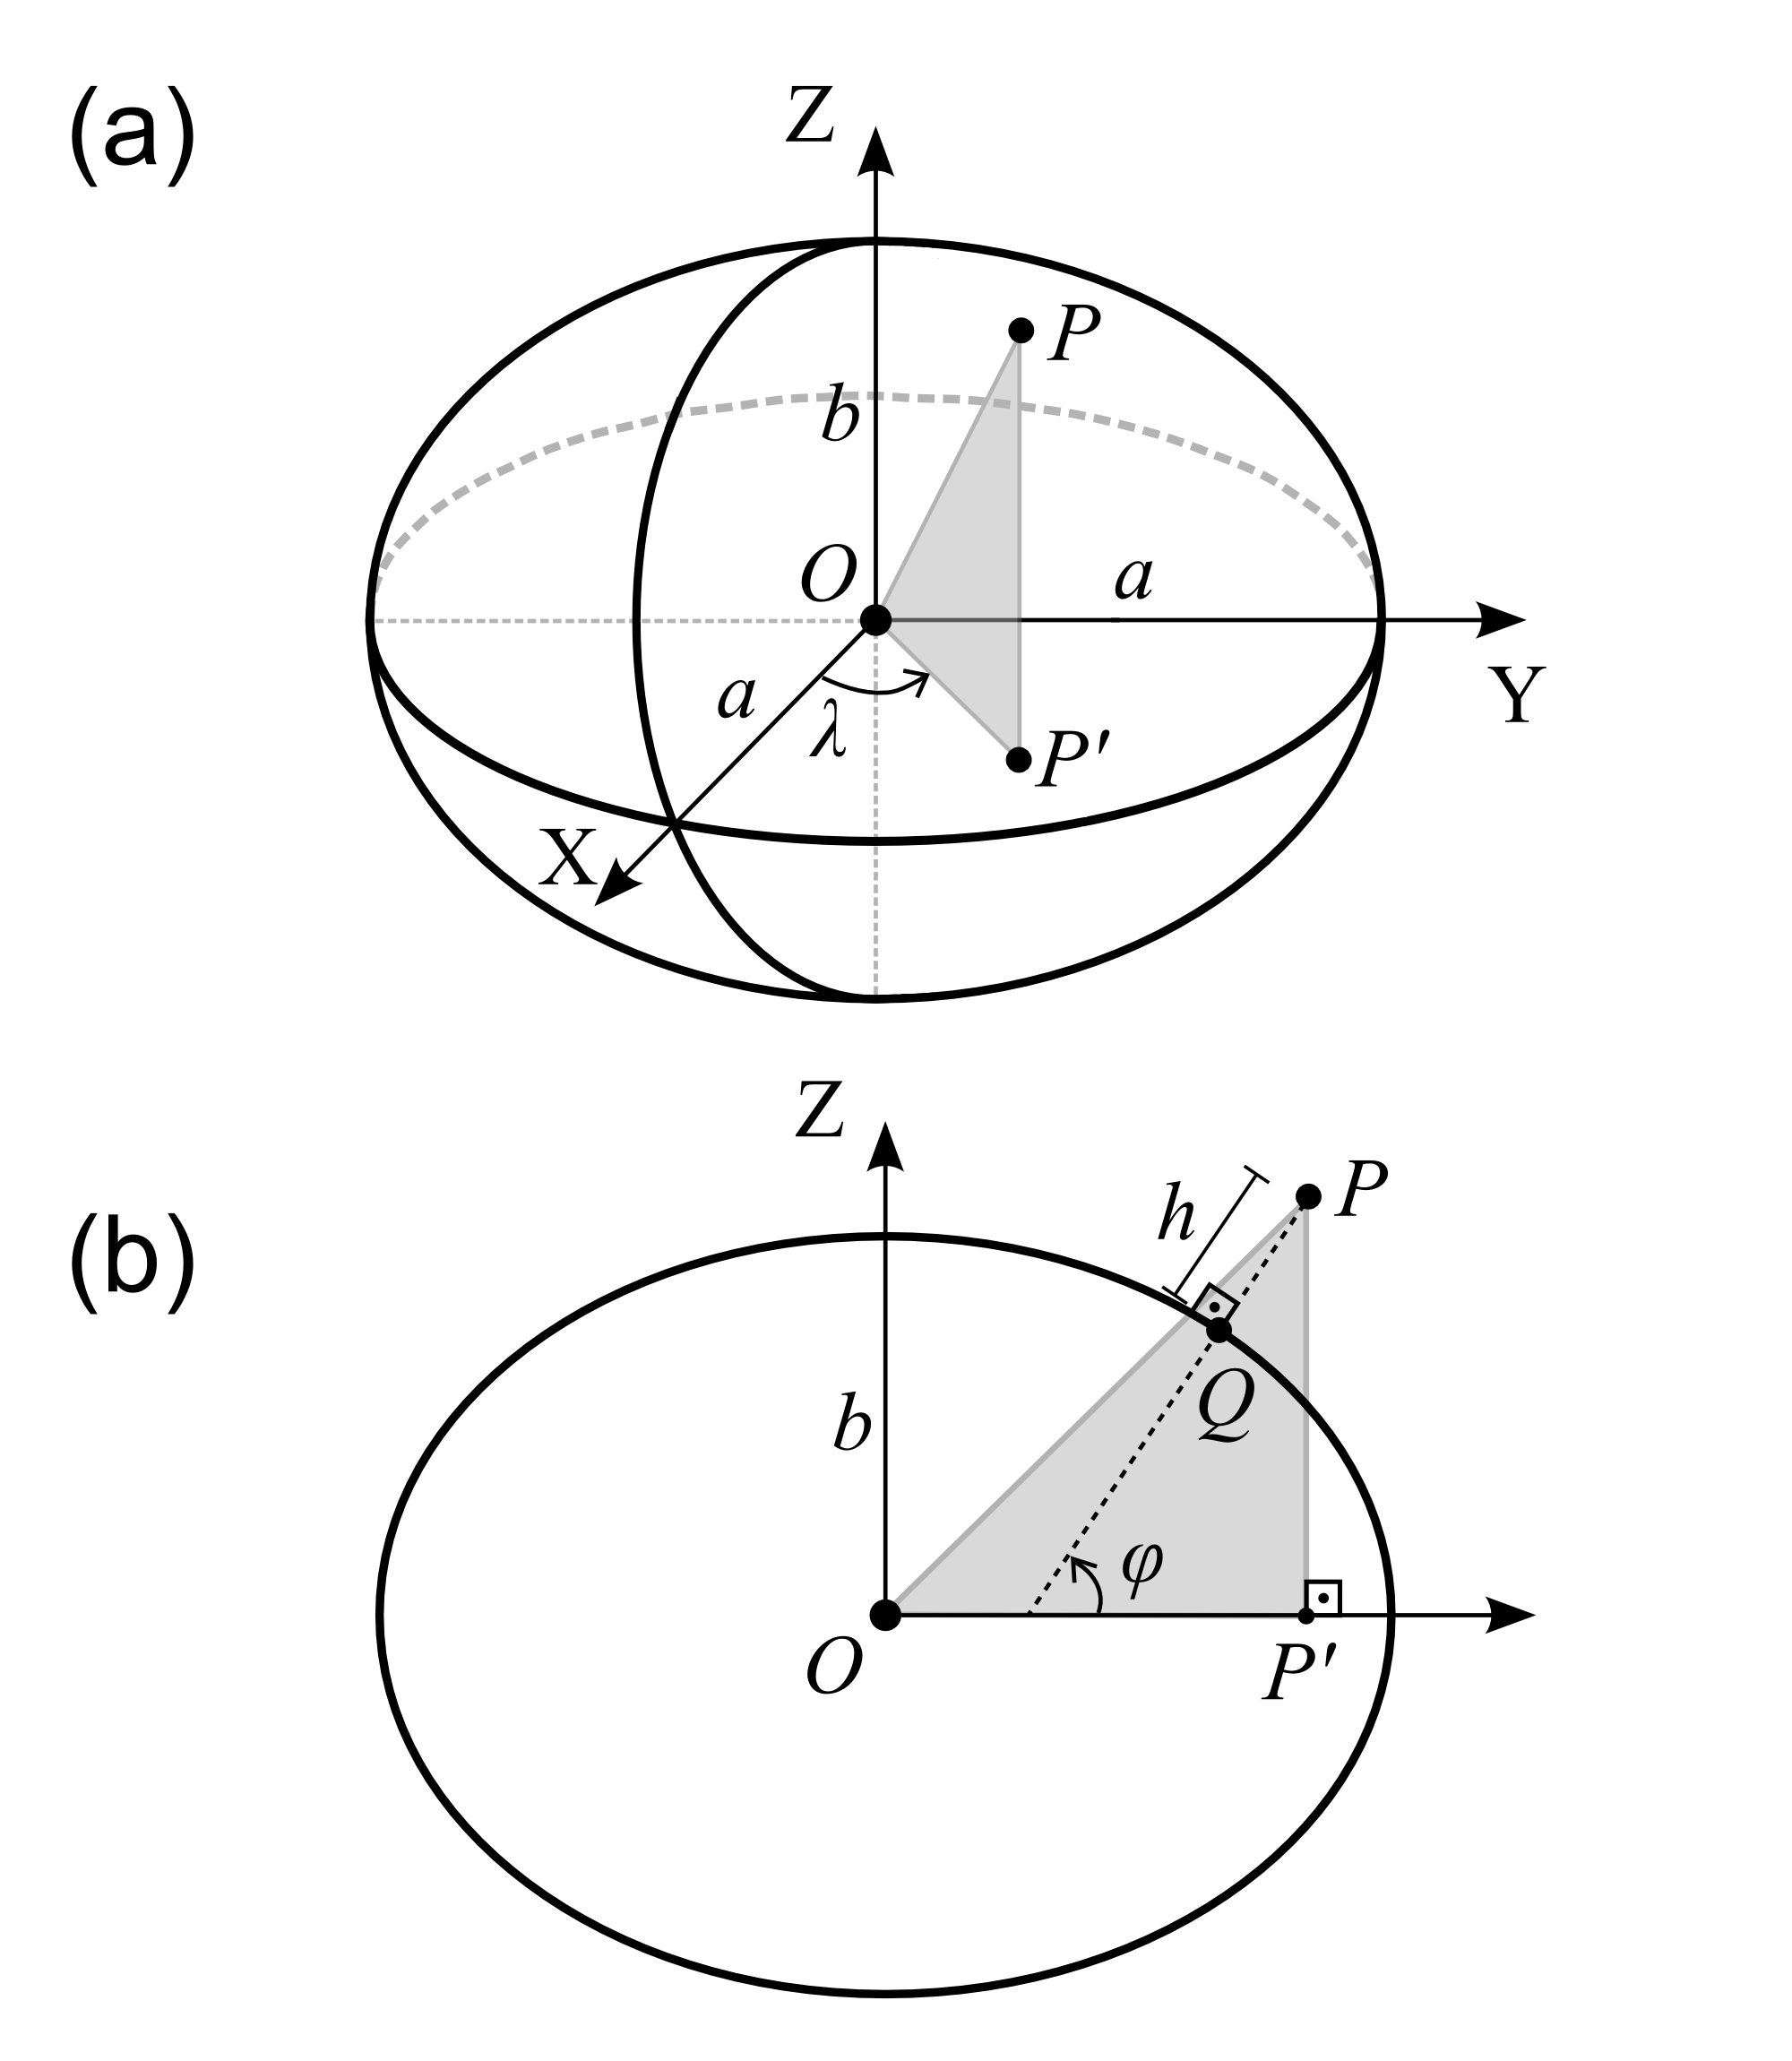
\includegraphics[width=0.3\textwidth]{figures/geodetic_coordinates.png}
    \caption{Schematic representation of the geodetic coordinate
    system.}
  \label{fig:fig1}
\end{figure}

\begin{figure}
    \centering
    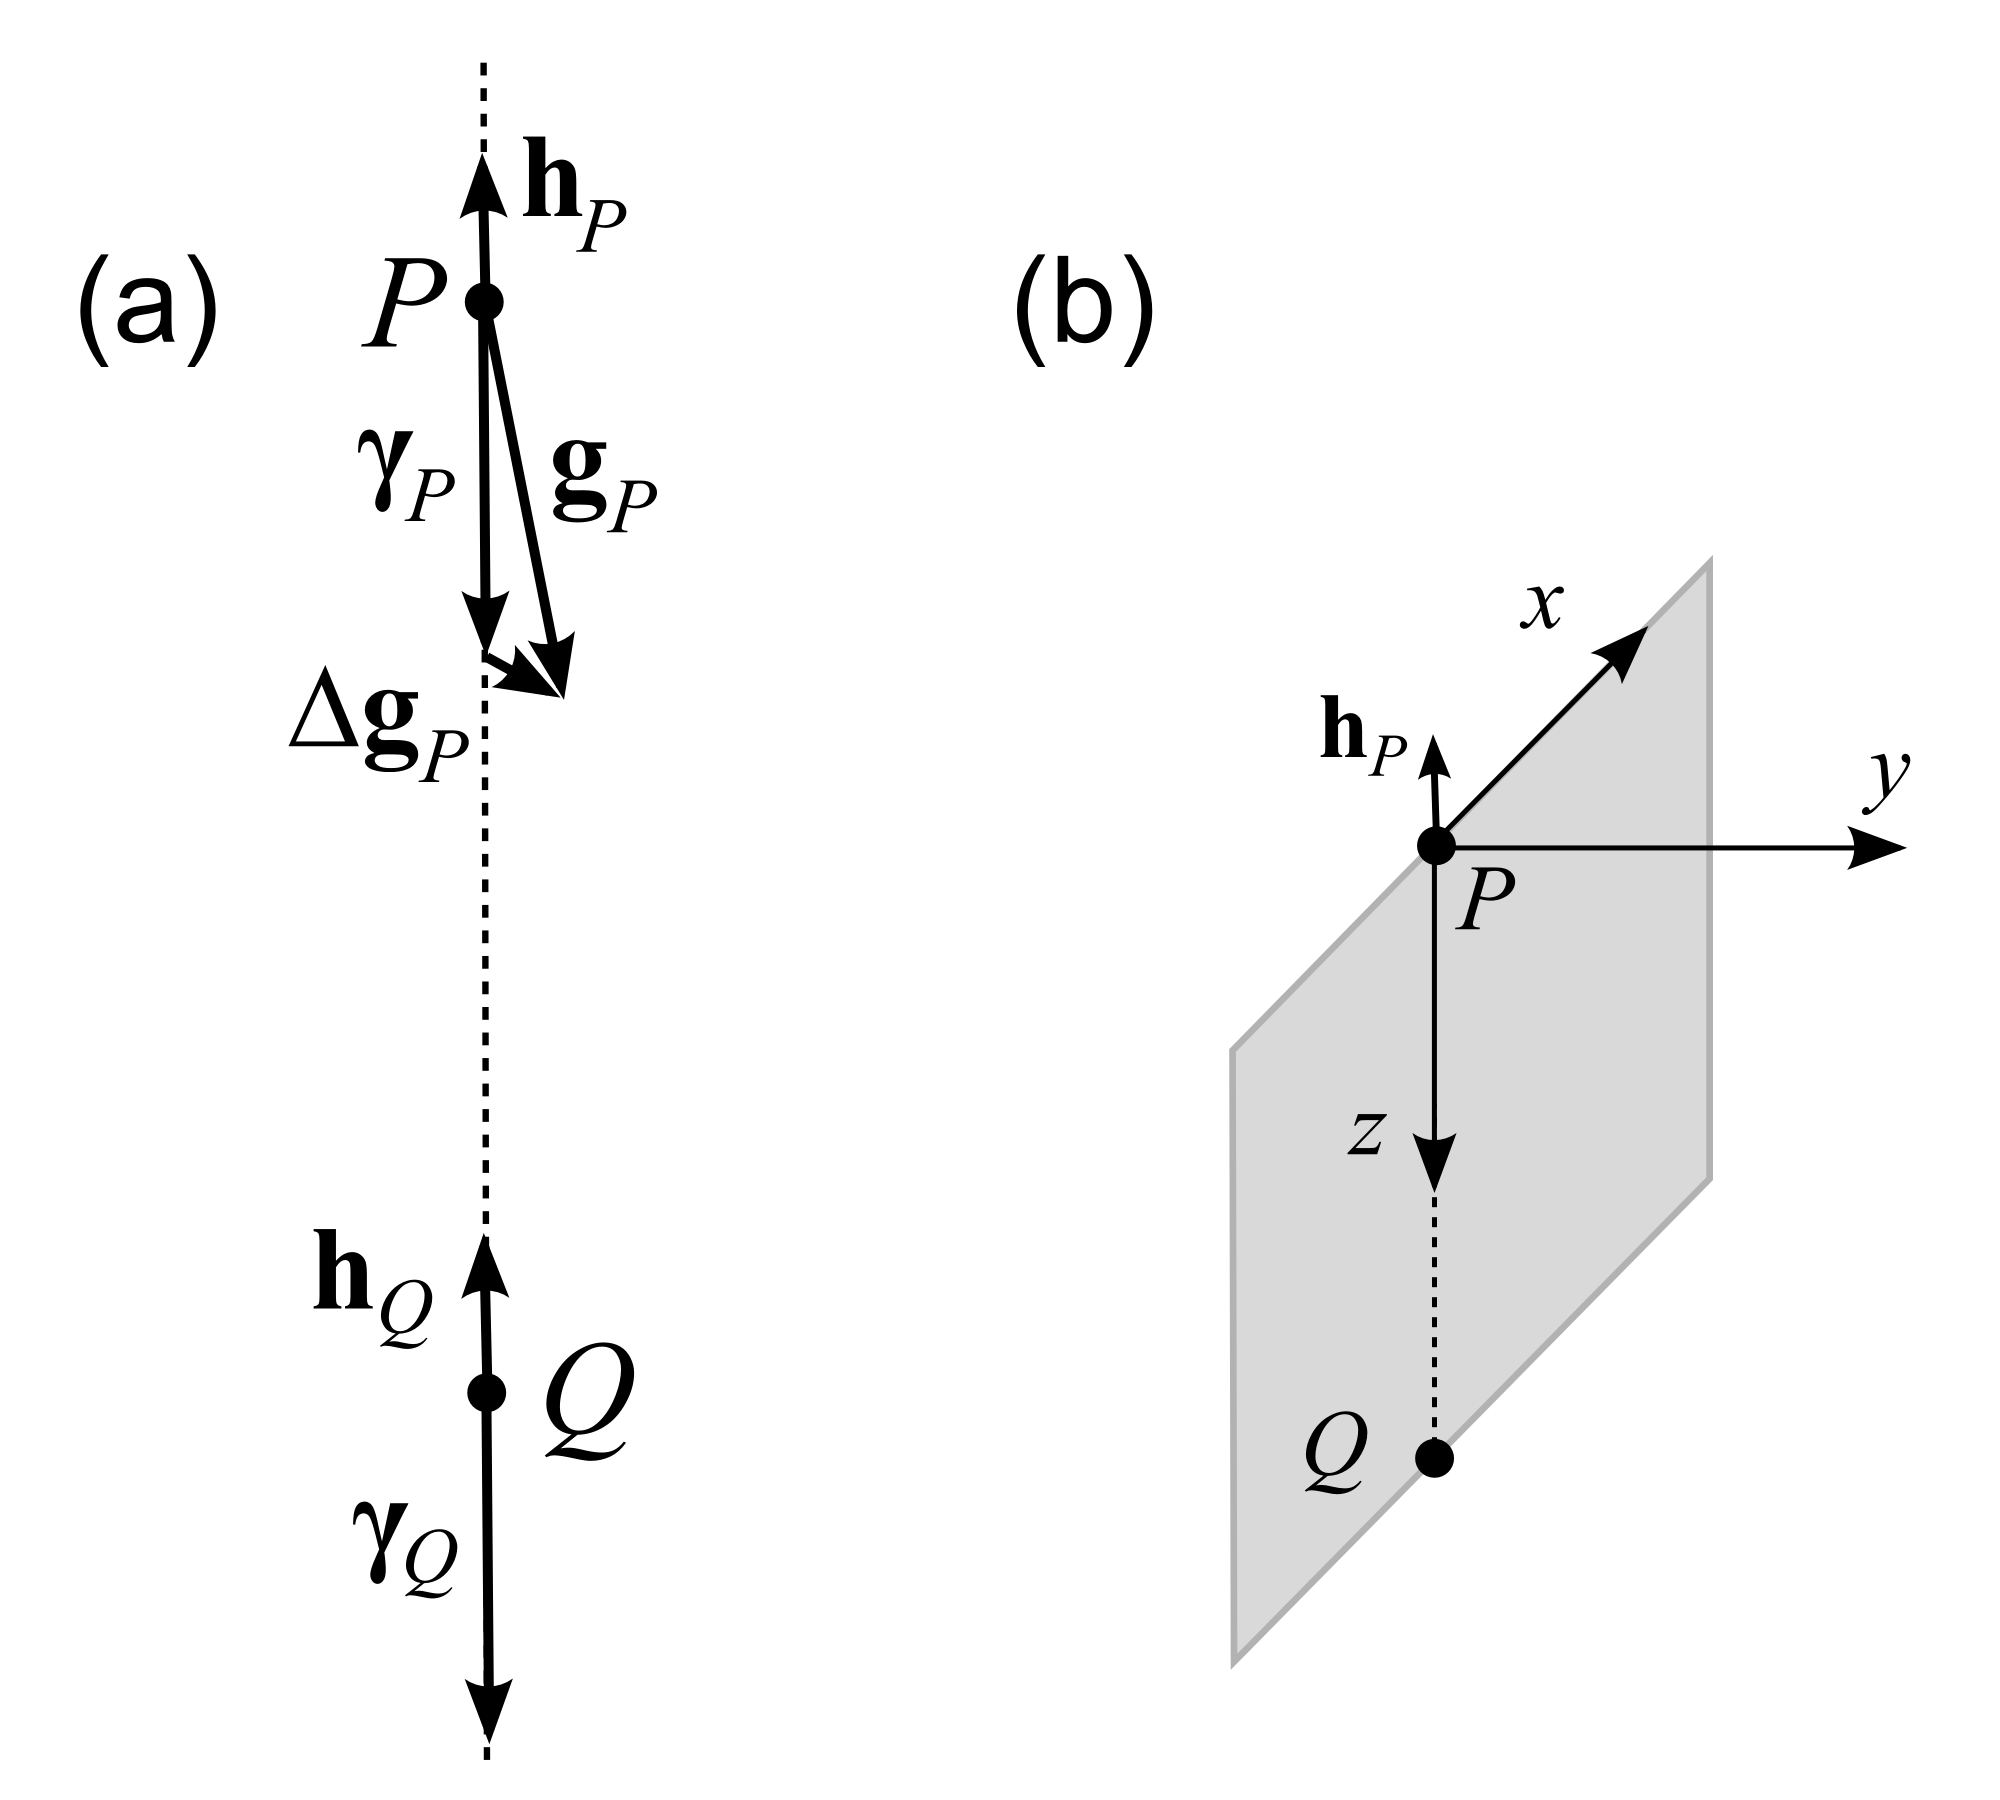
\includegraphics[width=0.3\textwidth]{figures/gravitational_disturbance.png}
    \caption{Schematic representation of the geodetic coordinate
    system.}
  \label{fig:fig2}
\end{figure}

\end{document}
